\chapter{Les différents modes}
\label{chap:différents modes}

Il existe plusieurs mode de fonctionnenement de l'AES, comme l'\aes.

\section{ECB - Electronic codebook}

Le mode ECB (Electronic codebook ou dictionnaire de code) est le plus simple. Il consiste à diviser le message à chiffrer en blocs qui vont être chiffrés indépendament des uns des autres. Pour le déchiffrement on procédera de la même manière en découpant le texte chiffré en bloc est en décryptant les blocs indépendament les uns des autres.

\begin{figure}[!h]
  \centering
  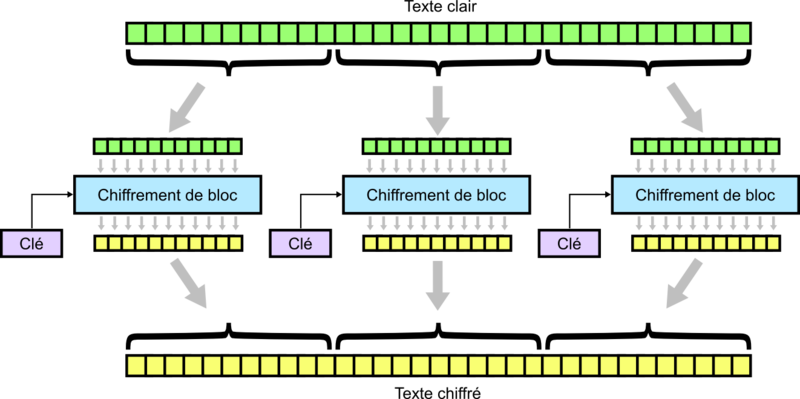
\includegraphics[width=\textwidth]{fonctionnement-ECB}
  \caption{schéma ECB \cite{wiki}}
  \label{schema ECB}
\end{figure}

Ce mode présente possède les avantages du chiffrement par flots, est pré-calculable et est parallélisable. Il offre la possibilité de déchiffrer une zone quelconque du texte chiffré et ainsi de déchiffrer une partie seulement des données.

Cependant ce mode possède un gros défaut est que deux blocs de texte clair seront chiffrés de la même manière, car il n'y a pas de randomisation. Ce défaut rend le mode ECB vulnérable aux attaques par dictionnaires et à l'analyse fréquentielle. En effet pour une clef donnée, on pourra générer un dictionnaire avec les correspondances entre les clair et le chiffré, permettant ainsi de retrouver le texte clair. Pour ces raisons l'utilisation de ce mode est fortement déconseillé.

\section{CBC}

Avec le mode CBC (Cipher Block Chainning ou Enchaînement des blocs) à chaque bloc de texte clair on applique un "XOR" (ou esclusif) avec le bloc chiffré précedent. Ainsi chaque bloc chiffré depend des bloc traité avant. Pour le premier bloc il faut fournir un vecteur d'initialisation.

\begin{figure}[!h]
  \centering
  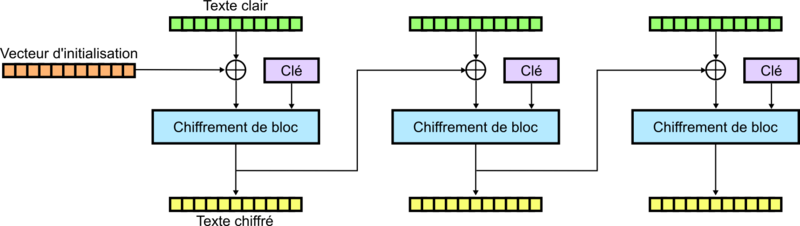
\includegraphics[width=\textwidth]{fonctionnement-CBC}
  \caption{schema CBC - Chiffrement \cite{wiki}}
  \label{schema CBC - Chiffrement}
\end{figure}

Ce mode présente possède les avantages du chiffrement par flots, et il offre également la possibilité de déchiffrer une zone quelconque du texte chiffré. Cependant un des incovénient et que le chiffrement est séquentiel ( \cad il ne peut pas être parallélisé).

Pour le déchiffrement, on passe le premier bloc crypté dans le déchiffrement de bloc et on effectue un "XOR" avec le vecteur d'initialisation IV. Remarque dans le cas ou le vecteur d'initialisation est incorrecte seul le premier bloc crypté sera impossible à decrypter. En effet à chaque bloc on applique un "XOR" avec le chiffrer du bloc précedent, et pas le texte clair. Ainsi on peut retrouver un bloc de texte claire uniquement a partir du bloc crypté précedent, ce qui permet ainsi la parallélisation de la décryption. 

\begin{figure}[!h]
  \centering
  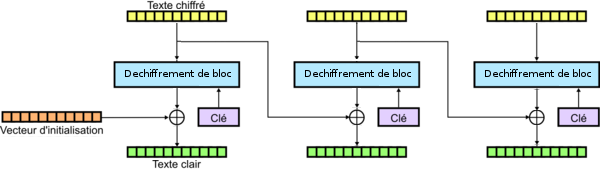
\includegraphics[width=\textwidth]{fonctionnement-CBC_de}
  \caption{schema CBC - Déchiffrement}
  \label{schema CBC - Déchiffrement}
\end{figure}




\section{CFB}
Le mode CFB (Cipher FeedBack ou Chiffrement à rétroaction) qui est similaire au mode CBC. Tout comme le CBC, ce mode permet de déchiffrer n'importeque zone du chiffré, cependant, comme le CBC, le chiffrement est séquentiel il ne peut donc pas être parallèlisé. Le déchiffrement est similaire au CBC est peu quant a lui être parallélisé. 

\begin{figure}[!h]
  \centering
  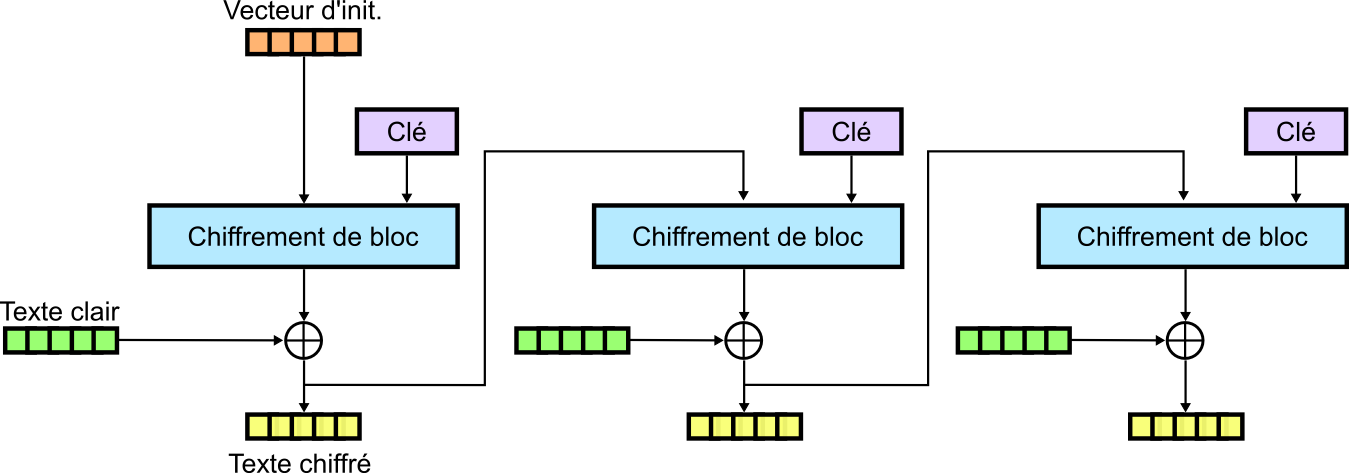
\includegraphics[width=\textwidth]{fonctionnement-CFB}
  \caption{schema CFB - Chiffrement}
  \label{schema CFB - Chiffrement}
\end{figure}

\begin{figure}[!h]
  \centering
  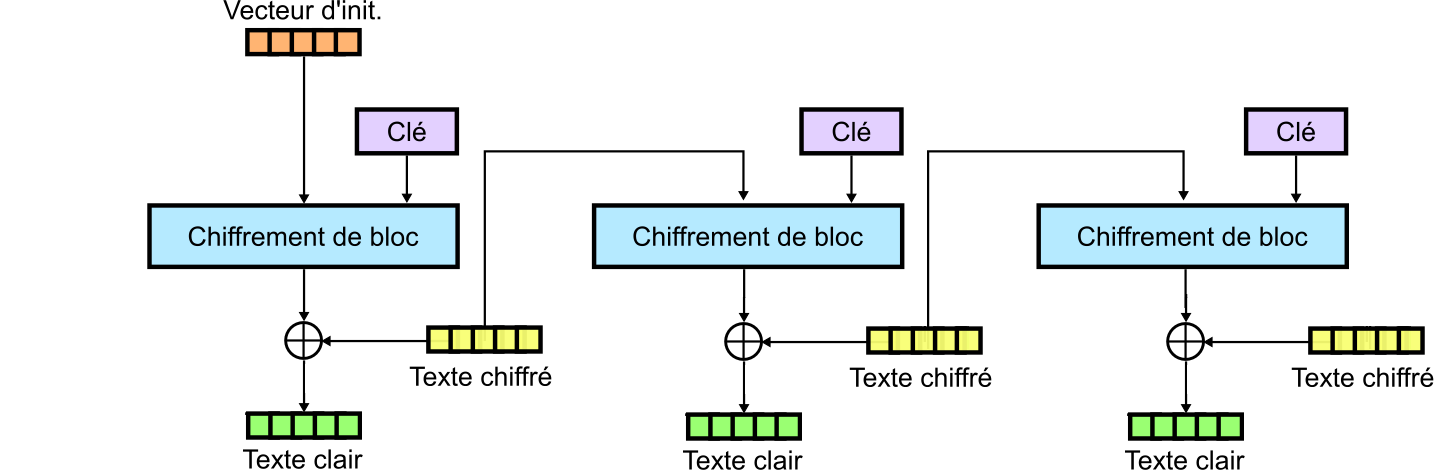
\includegraphics[width=\textwidth]{fonctionnement-CFB_de}
  \caption{schema CFB - Déchiffrement}
  \label{schema CFB - Déchiffrement}
\end{figure}

\section{OFB}
Le mode OFB (Output FeedBack) est une variante du mode CFB. En effet au lieu d'utiliser bloc chiffré pour chiffrer le suivant, le mode OFB va utiliser le chiffré du vecteur d'initialisation. S'il s'agit du bloc N, alors celui ci sera chiffrer avec le vecteur d'initialisation chiffré N fois. Le décryptage est très proche du CFB, il faut juste prendre le déchiffré du vecteur d'initialisation.


\begin{figure}[!h]
  \centering
  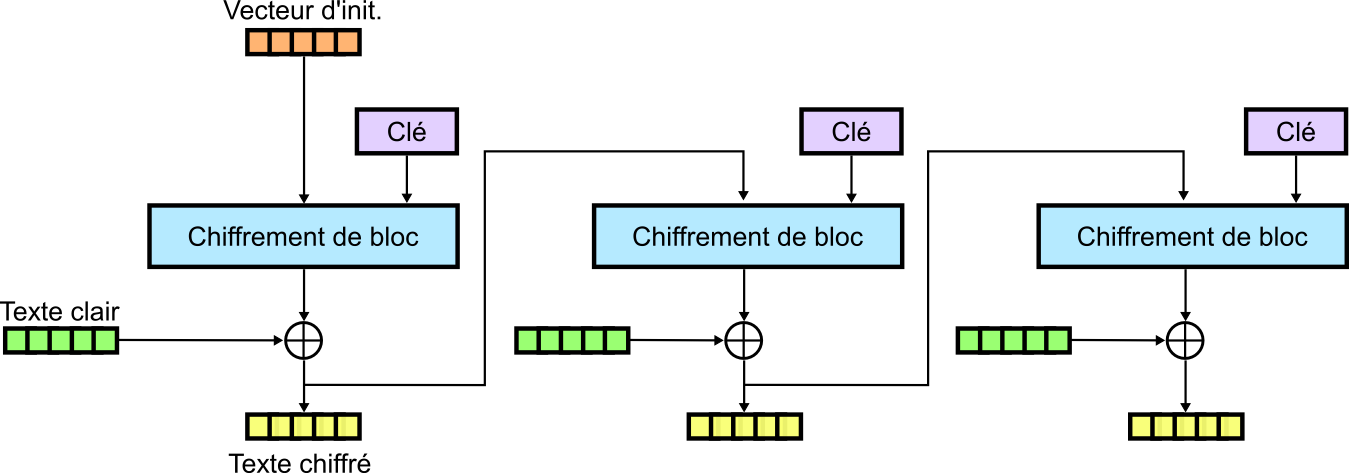
\includegraphics[width=\textwidth]{fonctionnement-OFB}
  \caption{schema OFB - Chiffrement}
  \label{schema OFB - Chiffrement}
\end{figure}

\begin{figure}[!h]
  \centering
  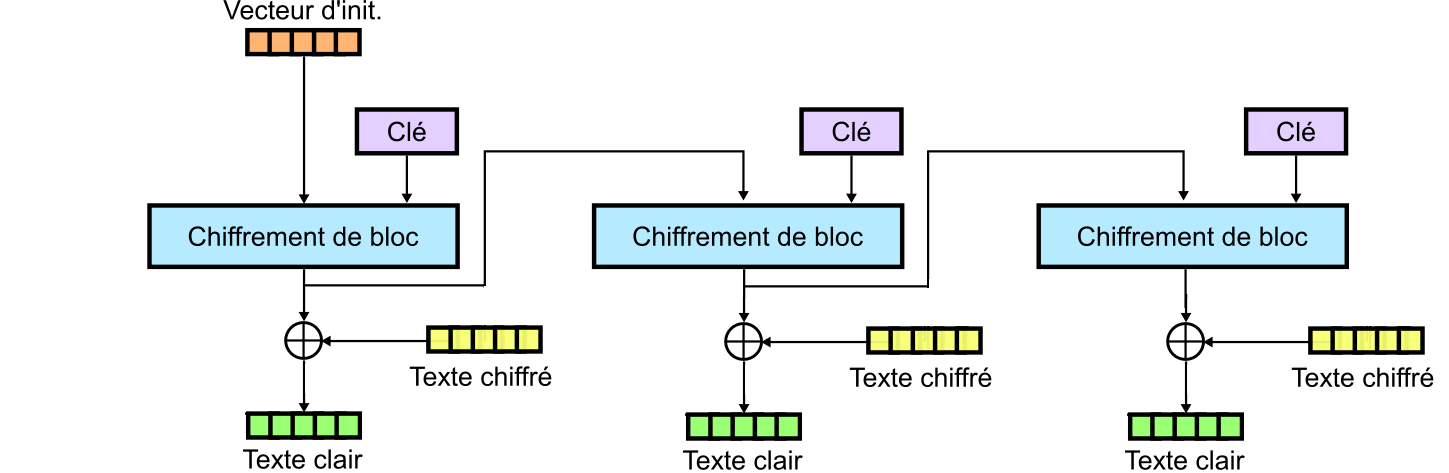
\includegraphics[width=\textwidth]{fonctionnement-OFB_de}
  \caption{schema OFB - Déhiffrement}
  \label{schema OFB - Déchiffrement}
\end{figure}

\section{CTR}





%%% Local Variables: 
%%% mode: latex
%%% TeX-master: "rapport_de_base"
%%% End: 
